%================================================================
\chapter{Results and Discussion}\label{chap:results_discussion}
%================================================================
In this chapter, we will detail how various models presented in previous chapters will be configured. We will also go into the spesifics on how the models will be characterized and investigated using aforementioned numerical methods. The results will be discussed and compared to earlier research as they are presented. 

In \autoref{sec:Vanishing Gradient Phenomenon}, the vanishing gradient phenomenon will be investigated for QNNs, QCNs and DNNs by studying how the magnitude of their gradients vary as a function of architecture. There will be put emphasis on the behaviour with respect to the number of layers.

In \autoref{sec:Investigating the Loss Landscape}, we will characterize the geometry of the loss landscape of QNNs, QCNs and DNNs by studying their EFIM spectrum, as presented in \autoref{sec:EFIM}. The result will be used to asses the trainability of different models and predict how architecture affects training.

In \autoref{sec:Expressivity}, we assess the expressivity of QCNs and compare them to DNNs, we will use trajectory length as presented in \autoref{sec:TrajectoryLength}. This will be done for both trained and untrained models.

In \autoref{sec:Training Models}, we test models in a practical setting, and give support to previous results and analyses in this thesis, by fitting them to gaussian data in multiple dimensions. This will be done both using idealised simulation(see \autoref{sec:Exact Expectation Value}), and simulated, noisy hardware(see).


%================================================================
\section{Vanishing Gradient Phenomenon}\label{sec:Vanishing Gradient Phenomenon}
%================================================================

%================================================================
\subsection{Vanishing Gradient in QNNs}\label{sec:Vanishing Gradient for QNNs}
%================================================================
We start by investigating the magnitude of the gradient for QNNs for different number of qubits and repetitions of the ansatz. To construct the QNNs, we use qubit encoding with $R_x$ rotations together with the simple ansatz. To derive an output, we estimate the parity of the state exactly using the methods outlined in see \autoref{sec:Exact Expectation Value} and \autoref{sec:Inference}. 
Instead of investigating the gradient of some loss function, i.e. \autoref{eq:LossDerivateWRTparameter}, we will investigate the gradient of the model output itself, $\frac{\partial f(\boldsymbol{x}^{(i)};\boldsymbol{\theta})}{\partial \theta_j}$. If this quantity vanishes, it follows that also \autoref{eq:LossDerivateWRTparameter} vanishes, for any loss function and labels $y^{(i)}$. To be concrete, we seek to compute the magnitude of the gradient averaged over the parameters and samples, i.e.
\begin{equation}
    \frac{1}{Nn_{\theta}}\sum_{i,j}\big|\frac{\partial f(\boldsymbol{x}^{(i)};\boldsymbol{\theta})}{\partial \theta_j}\big|
\end{equation}

To get a result representative of a realistic feature space, we will sample features $\mathcal{X} = \{\boldsymbol{x}^{(1)}, \cdots, \boldsymbol{x}^{(N)}\}$ uniformly as $\mathcal{X} \sim U(-\frac{\pi}{2}, \frac{\pi}{2})^{[N,p]}$. Here, we will use $N=100$ samples, and the number of features $p$ will be set equal to the number of qubits for each QNN. The QNNs will also be initialized in the standard way, i.e. sampling parameters as $\theta_j \sim U(-\pi, \pi)$. The resulting magnitude of the gradients for different number of qubits and ansatz repetitions can be seen in figure 

\begin{figure}[htp]
    \centering
    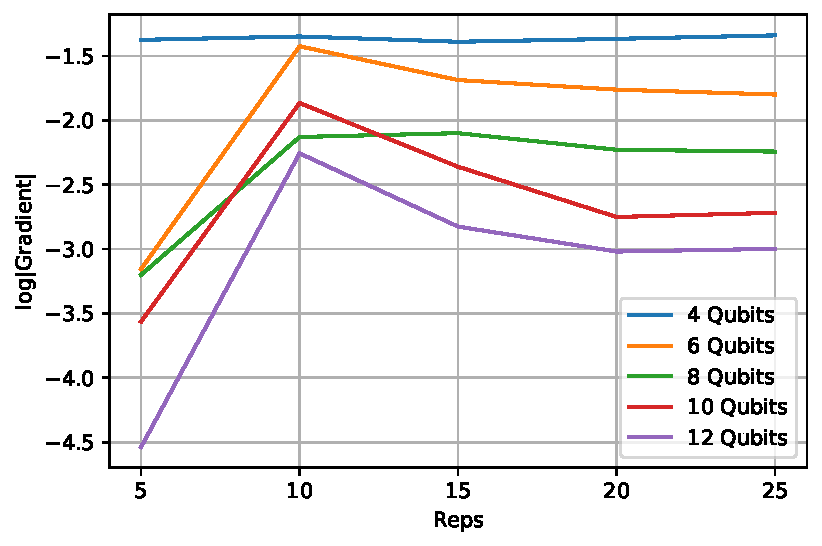
\includegraphics[width=12cm]{latex/figures/vanishing_gradient_QNN.pdf}
    \caption{}
    \label{fig:QNN_vanishing}
\end{figure}

From the above figure, we see that our implementation of QNNs results in a gradient that vanishes in the exponential regime with respect to the number of qubits. Also, the vanishing is worse the more repetitions of the ansatz is used. This behaviour can be explained by the fact that QNNs are a special case of PQCs. By encoding random inputs and randomly initializing the parameters, the QNN approaches essentially a random circuit. As shown by \citet{McClean_2018}, randomly initialized PQCs tend to produce gradients closely centered around zero as the number of qubits are increased. This is also consistent with our analysis of QNNs. As explained in \autoref{sec:BarrenPlateus}, it is necessary to use exponentially many shots in order to obtain a good signal-to-noise ratio for wide circuits, which in turn may make training intractable. 

%================================================================
\subsection{Vanishing Local Gradient in QCNs}\label{sec:Vanishing Local Gradients in QCNs}
%================================================================

A potentially promising feature of QCNs is the ability to scale up the model by introducing more circuits, rather than wider and deeper ones. As the gradient of QNNs tend to vanish for a high number of qubits, we want to investigate how the gradients of smaller QNNs behave when they enter as nodes in a QCN architecture. 

The QNNs used to contruct QCNs here are set up and initialized in the same manner as in \autoref{sec:Vanishing Gradient for QNNs}, with two repetitions of the simple ansatz. Also, we sample input data in the same manner, i.e. uniformly as $\mathcal{X} \sim U(-\frac{\pi}{2}, \frac{\pi}{2})^{[N,p]}$, with $N=100$ and the number of features $p$ set to the number of qubits used in the QNNs. In this section, all QCNs have 8 hidden layers an. Each hidden layer will utilize the number of nodes, $d$, which will range from $4$ to $8$. Also, the number of qubits in each node will be set to $d$ as well. Further, the outputs of each hidden layer is scaled to the interval $[-\pi, \pi]$ to make full use of the qubit encoding in the subsequent layer. \autoref{fig:QCN_local_vanishing} shows the magnitude of the local gradients \autoref{eq:localGradients} of the nodes, averaged over each layer, the samples and $10$ different realizations of the models. In addition, the standard deviation of this magnitude is estimated over the different realizations, yielding a confidence interval as seen in the figure. 

\begin{figure}[H]
    \centering
    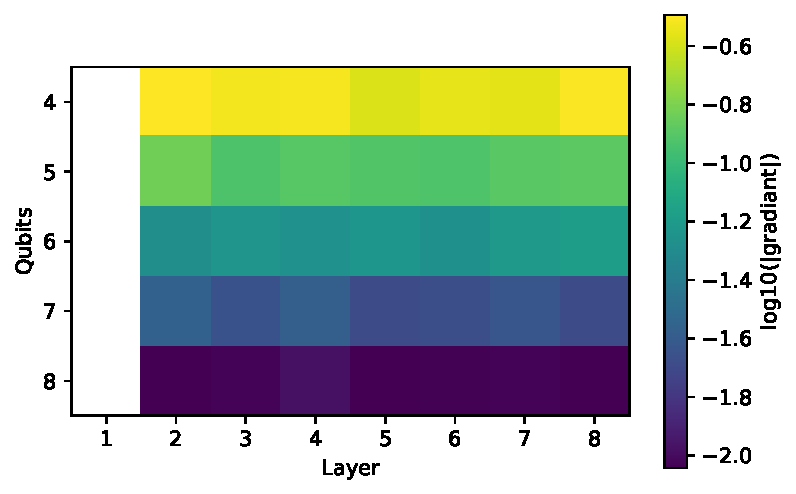
\includegraphics[width=12cm]{latex/figures/vanishing_gradient_partial_input.pdf}
    \caption{}
    \label{fig:QCN_local_vanishing}
\end{figure}

In the above figure we see the average magnitude of the local gradients for different layers and number of qubits. The local gradients of the QNNs entering the QCN model tend to vanish exponentially in the number of qubits, as with the single-circuit QNNs seen in \autoref{fig:QNN_vanishing}. However, the relative position of the QNNs along the depth of the QCN does not seem to affect the magnitude. This can be seen from the overlapping confidence intervals of the magnitudes for each number of qubits. Any variation of the average magnitude between the layers is thus likely just noise induced by the low number of $10$ parameter realizations, and does not indicate significant differences. This suggests that QCNs can be scaled up by making them deeper, with a computational cost linear in the number of layers, without affecting the magnitude of the local gradients. Consequently, a constant number of shots can be used for each node during estimation to obtain a certain single-to-noise ratio. 

%================================================================
\subsection{Vanishing Total Gradient in QCNs}\label{sec:Vanishing Total Gradients in QCNs}
%================================================================

In the previous section, it was shown that scaling up QCNs by adding more layers did not effect the number of shots needed to sufficiently estimate the local gradients of each QNN. This is in opposition to single-QNN models, whose gradient vanishes as both the number of qubits and repetitions are increase, as seen in \autoref{fig:QNN_vanishing}. However, we need to investigate how the magnitude of the total gradient \autoref{eq:derivweightsQCN} behaves as the number of layers is increased. In this section, the total gradient is calculated using the local gradients from the same numerical experiment as in \autoref{sec:Vanishing Local Gradients in QCNs}. As previously, the magnitude of the total gradient is averaged over each layer, the samples and 10 realisations of the parameters. \autoref{fig:QNC_vanishing_total} shows the average total gradient QCNs for each layer, for different number of qubits. For comparison, it also shows the magnitude of the total gradient of a DNN with the same number of layers and similar number of parameters as the biggest QCN.

\begin{figure}[H]
    \centering
    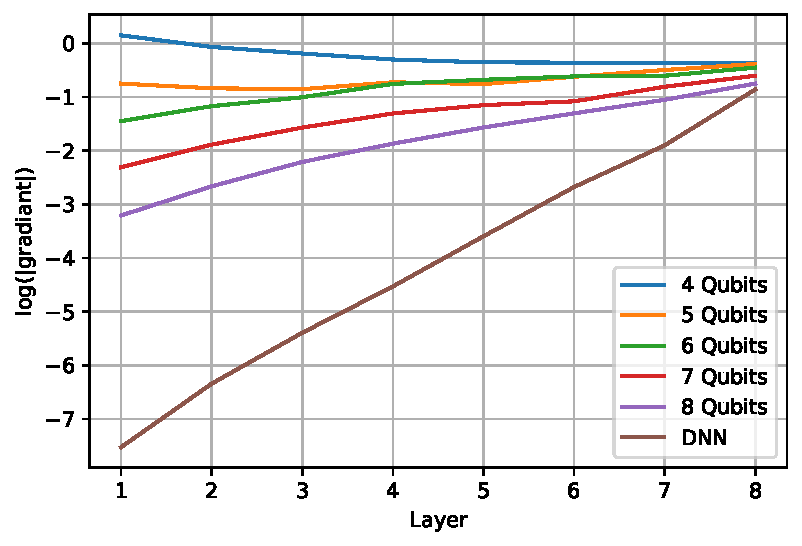
\includegraphics[width=12cm]{latex/figures/vanishing_gradient_total.pdf}
    \caption{}
    \label{fig:QNC_vanishing_total}
\end{figure}

From \autoref{fig:QCN_local_vanishing}, we see that the total gradient for a given layer of the DNN tends to vanish exponentially in the number of layers after it. This is a well-known phenomenon for classical neural networks, often explained by the saturation of the activation function during feed forward\cite{shalevshwartz2017failures}. As the activations tend to be very flat for when saturated, as for the sigmoid function used here, the gradient tends vanish during back propagation.

As with the DNN, also the QCNs exhibits vanishing total gradient with increasing number of layers, with a strong dependence on the number of qubits in each node. Seen in \autoref{fig:QCN_local_vanishing}, the total gradient vanishes faster for higher number of qubits in each node. This phenomenon can be related to the magnitude of the local gradients. As the error of the QCN is propagated backwards using \autoref{eq:errorQCN}, it accumulates the local gradients $\frac{\partial \boldsymbol{a}^{l+1}_k}{\partial \boldsymbol{a}^{l}_j}$ as factors. In the case that these factors are large, the error will tend to decrease slowly, and hence also the total gradient by \autoref{eq:derivweightsQCN}. This is the case for architectures with few qubits per node, as discussed in \autoref{sec:Vanishing Local Gradients in QCNs}. However, as the number of qubits increase, the local gradients will tend to decrease. Accumulating small factors will causes the error to decrease faster, exponentially so for each layer. In a sense, this vanishing of local gradients with increasing number of qubits is analogous to the saturation of the activations for classical networks.

Even though the magnitude of local gradients of QCNs tends to stay constant in the number of layers, we saw that back propagation induce an exponentially vanishing gradient. Although this behaviour is similar to that of DNNs, it is not as severe for the architectures used in this section: For the largest QCN of 100 parameters, the magnitude of the total gradient for the first layer is of order $10^{-3}$, as opposed to $10^{-7.5}$ for the DNN. Obviously, this difference will tend to decrease when increasing the number of qubits. 

An interesting observation is that the vanishment caused by back propagation happens in a purely classical part of the optimization, with the local gradients stored as floating-point numbers. This means that even though the total gradient tends to decrease exponentially with the number of layers, it does not introduce an exponential overhead on the quantum computer by requiring more shots. This is true, however, for single-QNN models as discussed in \autoref{sec:BarrenPlateus}. Put another way, QCNs' use of several smaller circuits, rather than one big, moves the estimation of vanishing quantities (the gradient) from quantum expectation values to classical computation.       

%================================================================
\section{Investigating the Loss Landscape}\label{sec:Investigating the Loss Landscape}
%================================================================
We explore the geometry of the loss landscape of various models by studying the eigenvalue spectrum of the EFIM. Looking \autoref{eq:EmpiricalFisher}, we see that the EFIM, unlike the Hessian, is independent of targets $y^{(i)}$. This makes the analysis problem independent, and serves to characterises architectures only. The input data $\mathcal{X} = \{\boldsymbol{x}^{(1)}, \cdots, \boldsymbol{x}^{(N)}\}$, used for calculating the EFIM, is sampled randomly from a standard normal distribution as $\mathcal{X} \sim N(0,1)^{(N,p)}$. This ensures that the input is evenly sampled from feature space and is consistent with the analysis of \citet{abbas2020power}.  Here, we use $N=200$ samples and either $p=4$ or $p=6$ inputs, depending on the model. For each unique model, the EFIM is calculated 10 times for different random initializations of the parameters(see stuff). The resulting spectrum is then averaged over the 10 initializations to produce more significant results. For a complete description of the models analysed in this section, see \autoref{tab:FIM models}.

\begin{table}[H]
\centering
\begin{tabular}{|l|l|l|l|l|l|l|l|}
\hline
Model &Type & Qubits& Reps & Layers & Width & Encoder        & $n_{\theta}$ \\ \hline
A    & QNN & 4& 18   & 1      & 4     & RZZ Encoding   & 72  \\ \hline
B    & QCN & 4& 3    & 2      & 4     & Qubit Encoding & 60 \\ \hline
C    & QCN & 4& 2    & 3      & 4     & Qubit Encoding & 72  \\ \hline
D    & QCN & 4& 1    & 5      & 4     & Qubit Encoding & 68  \\ \hline
E    & DNN & NA& NA   & 3      & 6     & NA             & 79 \\ \hline
F    & QNN & 6& 26   & 1      & 6     & RZZ Encoding   & 156  \\ \hline
G    & QCN & 6& 4    & 2      & 6     & Qubit Encoding & 168 \\ \hline
H    & QCN & 6& 2    & 3      & 6     & Qubit Encoding & 156  \\ \hline
I    & QCN & 6& 1    & 5      & 6     & Qubit Encoding & 150  \\ \hline
J    & DNN & NA& NA   & 3      & 9     & NA             & 163 \\ \hline
\end{tabular}
\caption{Description of the architecture of the models analysed in this section. The QNN and QCN models use exact evaluation of parity to derive outputs (see \autoref{sec:Exact Expectation Value} and \autoref{sec:Inference}). The DNN models uses sigmoid activation in all layers. The parameters of the models are appropriately initialized as presented in (stuff).} 
\label{tab:FIM models}
\end{table}

\autoref{fig:FIM Comparison} compares the EFIM spectrum of QNNs, QCNs and DNNs. Their architectures are chosen so that the models have approximately equal number of parameters. This is to ensure a fair comparison. Looking at the spectra of the DNN models, we see the characteristic result of a singular large eigenvalue, with the rest sitting close to zero. This indicates that DNN models exhibit a loss landscape that is very flat in all but one direction, where it is extremely distorted. This result is consistent with the findings of \citet{abbas2020power} and \citet{karakida2019universal}. As explained in \autoref{sec:Optimization}, this geometry of the loss landscape is often associated with slower optimization. Further, we see that the spectra of the our QNN models are much more uniformly distributed compared to the DNN models. This results in a loss landscape that is significantly distorted in most directions, rather than just one. \citet{abbas2020power} came to the same conclusion for their QNN models, and argued that this uniformity of the spectrum meant that landscape was more well-condition for optimization. They strengthened this hypothesis by showing numerically that QNNs trained faster than DNNs. 

\begin{figure}[H]
    \centering
    \begin{subfigure}[t]{0.5\textwidth}
        \centering
        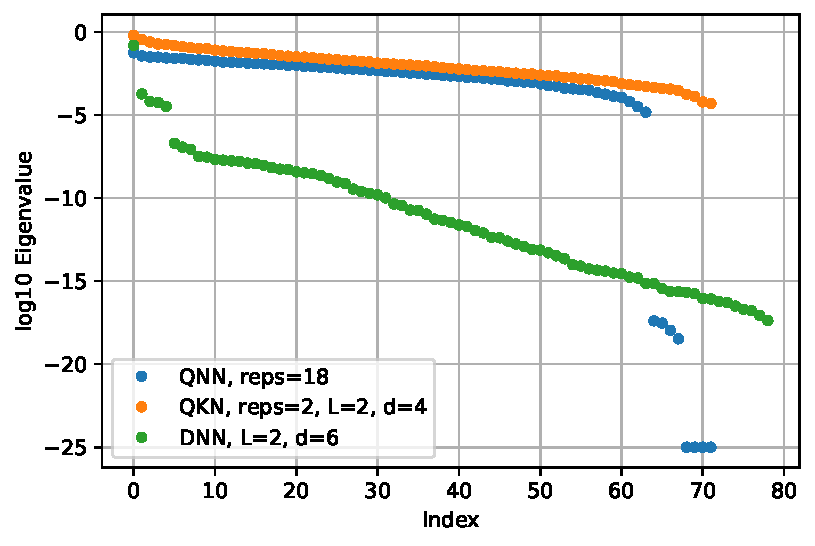
\includegraphics[height=1.9in]{latex/figures/FIM_qubits_4.pdf}
        \caption{Lorem ipsum}
        
    \end{subfigure}%
    ~ 
    \begin{subfigure}[t]{0.5\textwidth}
        \centering
        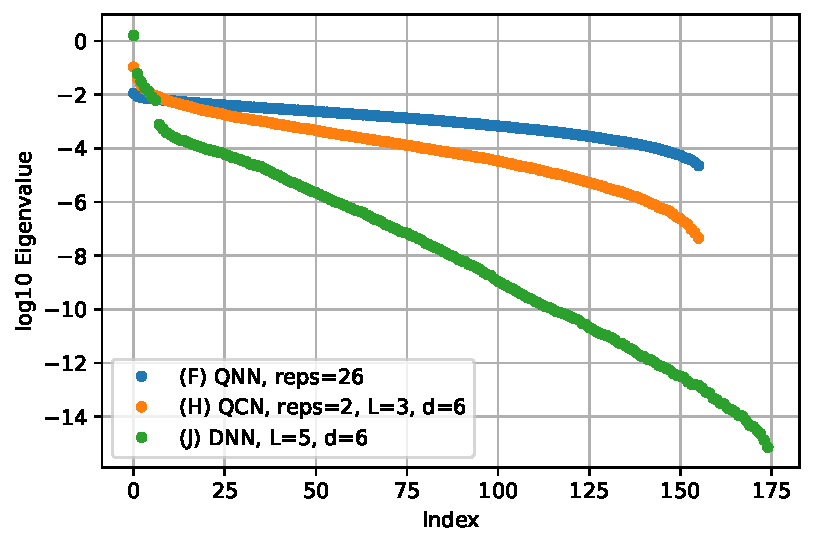
\includegraphics[height=1.9in]{latex/figures/FIM_qubits_6.pdf}
        \caption{Lorem ipsum}
    \end{subfigure}
    \caption{Caption place holder}
    \label{fig:FIM Comparison}
\end{figure}

Returning to \autoref{fig:FIM Comparison}, we see that the spectra of the three layer QCNs exhibit much the same uniformity as the QNNs. A more thorough comparison between different QCNs can be seen in \autoref{fig:FIM QCN}. In this figure, we vary the number of layers of the QNCs and the number of repetitions (i.e. the number of times the ansatz is repeated for each node), while keeping the total number of parameters roughly constant. In doing this, we get to precisely shift how much of the complexity of a given QCN results from the complexity of each node or overall structure of the network. \autoref{fig:FIM QCN a} shows that, for 4 qubit circuits, the spectra of the QNN and different QCNs exhibit roughly the same uniformity. Going up to 6 qubits,  \autoref{fig:FIM QCN b} shows that the spectrum tends to concentrate more around zero the more layers the QCN have. This is likely related to the vanishing of the gradient induced by back propagation. For 4 qubits, this is not as big of a problem since the local gradients are relatively big. However, for 6 qubits, the local gradients are smaller. This results in the gradient vanishing faster when increasing the number of layers, which in turn results in a flatter landscape. At any rate, even for the 5 layer QCN, the landscape is not as badly distorted as for the 5 layer DNN. Further, the few layered QCNs, in particular(ost). 


\begin{figure}[H]
    \centering
    \begin{subfigure}[t]{0.5\textwidth}
        \centering
        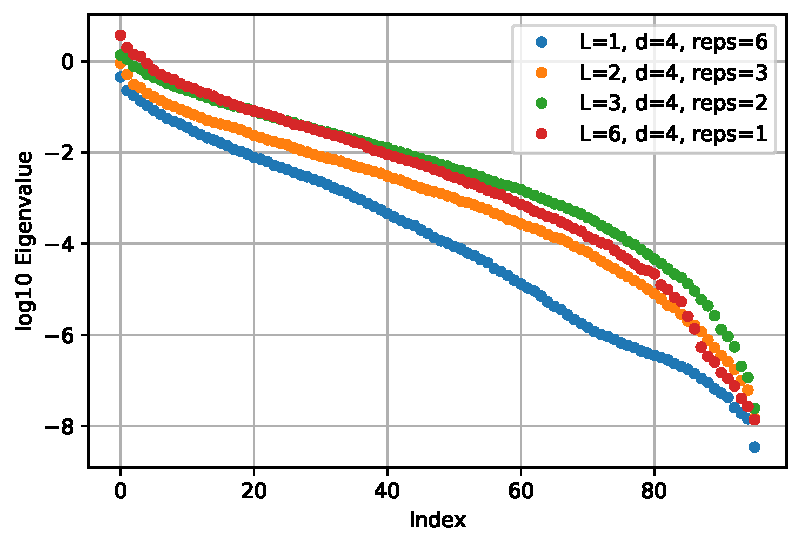
\includegraphics[height=1.9in]{latex/figures/FIM_qubits_4_comparison.pdf}
        \caption{Lorem ipsum}
        \label{fig:FIM QCN a}
    \end{subfigure}%
    ~ 
    \begin{subfigure}[t]{0.5\textwidth}
        \centering
        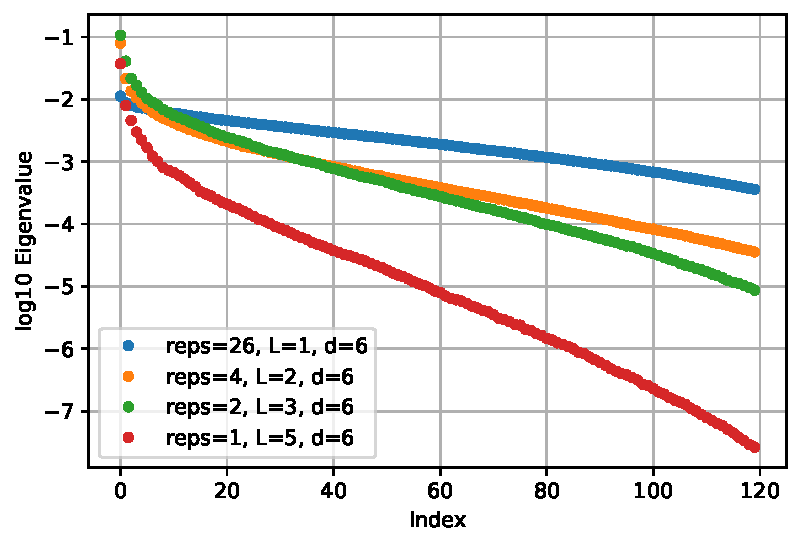
\includegraphics[height=1.9in]{latex/figures/FIM_qubits_6_comparison.pdf}
        \caption{Lorem ipsum}
        \label{fig:FIM QCN b}
    \end{subfigure}
    \caption{Caption place holder}
    \label{fig:FIM QCN}
\end{figure}


%================================================================
\section{Expressivity}\label{sec:Expressivity}
%================================================================
We will investigate the expressivity QCN using the trajectory length method of \citet{raghu2017expressive}, as described in \autoref{sec:TrajectoryLength}. The trajectory length will be first studied for randomly initialized QCNs for varying number of qubits in each node. Then, for some selected QCNs, the trajectory length will be investigated as the models are gradually fitted on 2D gaussian data. The results in both cases will be compared to similar DNNs, with approximately the same number of parameters for fair comparison. The input trajectory $\boldsymbol{x}(t_i)$ used will be circle in $\mathbb{R}^2$ with radius $\frac{\pi}{2}$ and centered around $0$, divided up into $1000$ equally spaced point.

%================================================================
\subsection{Untrained Models}\label{sec:Untrained Models}
%================================================================

\autoref{fig:TL_untrained} shows the trajectory length resulting from each layer up to the eighth laye, for several different QCNs. All layers have $d$ number of nodes, and all nodes have $d$ number of qubits. $d$ ranges from $4$ to $8$. For comparison, the trajectory length is also calculated for an 8-layer DNN with approximately the same number of parameters as the biggest QCN. The QCNs and the DNN is randomly initialized, as in \autoref{sec:Vanishing Gradient Phenomenon}.

\begin{figure}[htp]
    \centering
    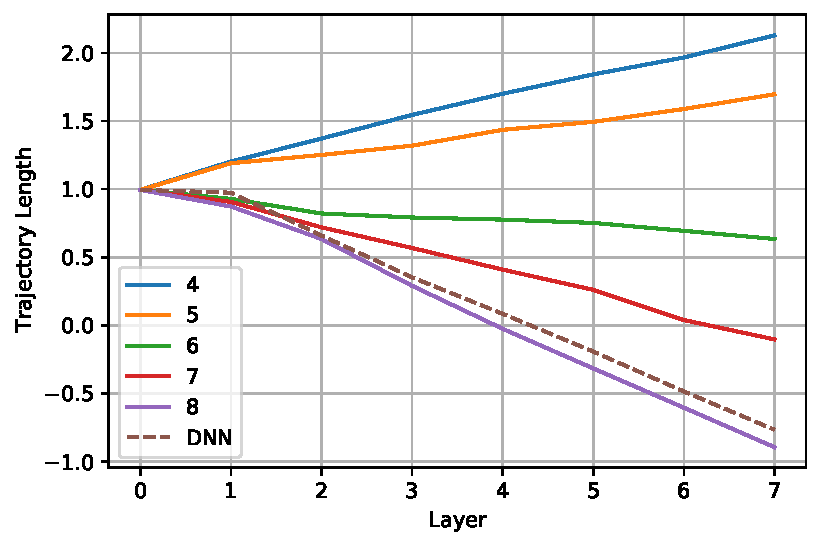
\includegraphics[width=12cm]{latex/figures/TL_untrained.pdf}
    \caption{}
    \label{fig:TL_untrained}
\end{figure}

\autoref{fig:TL_untrained_projection}, accompanying \autoref{fig:TL_untrained}, shows the trajectories of selected models and layers, projected onto 2D. The rows correspond to the 4 qubit QCN, 8 qubit QCN and DNN, from top to bottom. The columns correspond to the first layer, second layer, third layer and last layer, left to right.   

\begin{figure}[htp]
    \centering
    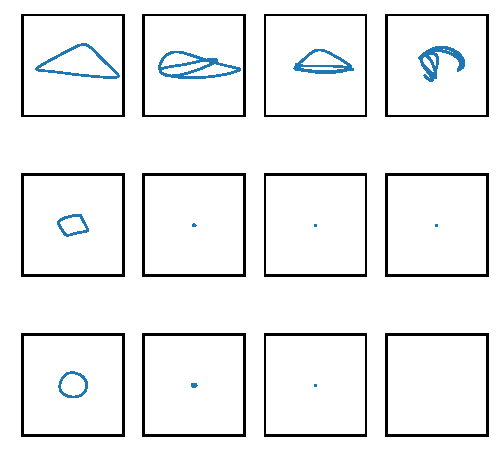
\includegraphics[width=12cm]{latex/figures/TL_untrained_projection.pdf}
    \caption{}
    \label{fig:TL_untrained_projection}
\end{figure}

\autoref{fig:TL_untrained}, we see that the untrained DNN exhibits an exponential decrease in trajectory length as it is being transformed by each layer. From \autoref{fig:TL_untrained_projection}, we see this manifesting itself as the trajectory concentrating around some mean, progressively more for each layer. This shows that randomly initialized DNNs can tend to compute functions which are not very sensitive to the input, which is consistent with the result of \citet{raghu2017expressive}. 

From the same figures we see that the 4-qubit QCNs exhibits a trajectory length that increases approximately exponentially in the number of layers. \autoref{fig:TL_untrained_projection} shows how the trajectory changes after each layer for the same model, becoming increasingly more distorted and complex. This is in opposition of the result for the DNN, which rather showed an exponential decrease of the trajectory length, concentrating its trajectory around a mean. However, as the number of qubits in each node increase, the QCNs tend to produce trajectory lengths that decrease exponentially in the number of layers. This effect is more severe the more qubits are used. This effect can be explained by the concentration of output values of PQCs and QNNs and their mean, for increasing number of qubits. As QCNs create new features for each layer using QNNs, this concentration around the mean is applied multiple times, mapping the inputs closer and closer. 

For 4 though 8 qubits, the previous result indicates that QCNs generally compute more complex functions than the DNN when randomly initialized. A possible explanation for this is that the mathematical transformation applied by each QNN in each nodes are in a way more powerful and "interesting" compared to DNNs. As the information is represented as an entangled state in an exponentially large Hilbert space, each Pauli rotation transforms an exponential number of amplitudes. This constitutes a more complex computation than the affine transformation happening in the DNN, for the same number of parameters. However, this results only in a more interesting output for a low number of qubits, as the increased dimension of the Hilbert space tends to concentrate the output around the mean. 


%================================================================
\subsection{Trained Models}\label{sec:Trained Models}
%================================================================
\autoref{fig:TL_trained} shows how the trajectory length changes as various models are incrementally trained to fit 2D Gaussian data(see). The models being investigated here are two QCNs with 5 and 6 qubits, respectively, with each node QNN having the same architecture as in \autoref{sec:Untrained Models}. These will be compared with DNNs with approximately same number of parameters. For more information about the models, see \autoref{tab:TL models}. All the models are trained using Adam optimizer with the standard hyperparameters and a learning rate of $0.1$. The QCNs are trained for a total of $40$ and $60$ epochs, respectively, in increments of $10$. In order to produce a fair comparison, the DNNs will not be trained for the same increments of epochs. Rather, they will trained until they achieve approximately the same MSE on the training set as the QCNs, for each increment. In this way, we get to compare the expressivity of QCNs and DNNs that fit the data to an equal degree. 

\begin{figure}[H]
    \centering
    \begin{subfigure}[t]{0.5\textwidth}
        \centering
        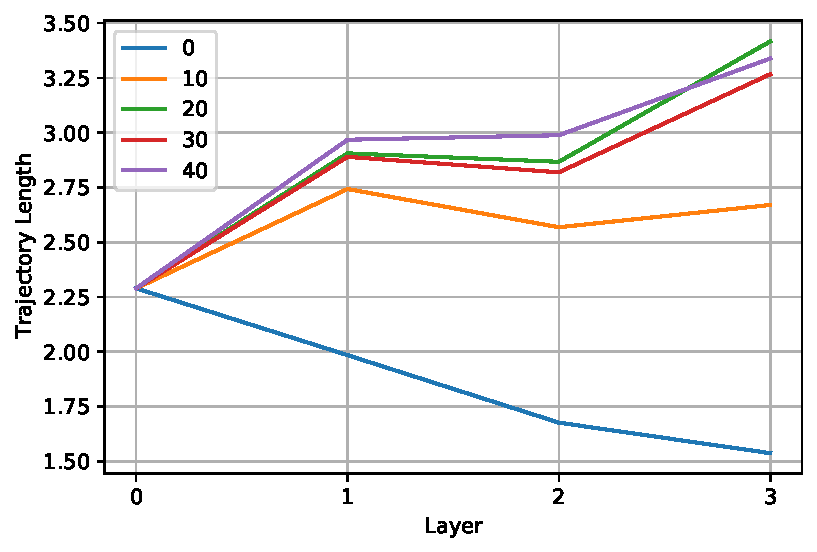
\includegraphics[height=1.9in]{latex/figures/TL_trained_QCN_qubit_5.pdf}
        \caption{Lorem ipsum}
        
    \end{subfigure}%
    \hfill 
    \begin{subfigure}[t]{0.5\textwidth}
        \centering
        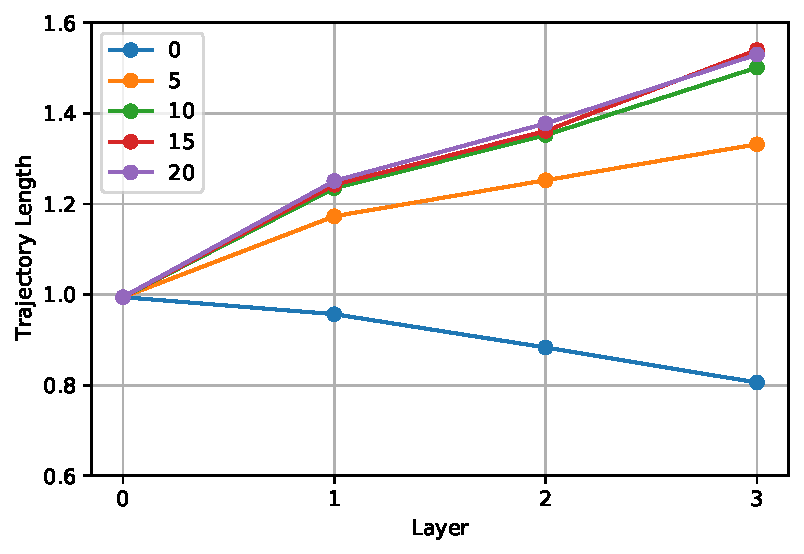
\includegraphics[height=1.9in]{latex/figures/TL_trained_QCN_qubit_6.pdf}
        \caption{Lorem ipsum}
    \end{subfigure}
    \vskip\baselineskip
    \begin{subfigure}[t]{0.5\textwidth}
        \centering
        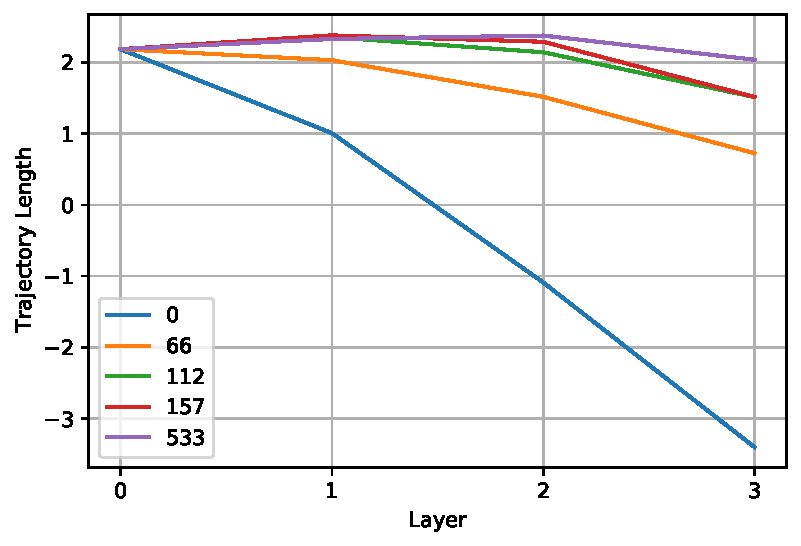
\includegraphics[height=1.9in]{latex/figures/TL_trained_DNN_nodes_8.pdf}
        \caption{Lorem ipsum}
        
    \end{subfigure}%
    \hfill 
    \begin{subfigure}[t]{0.5\textwidth}
        \centering
        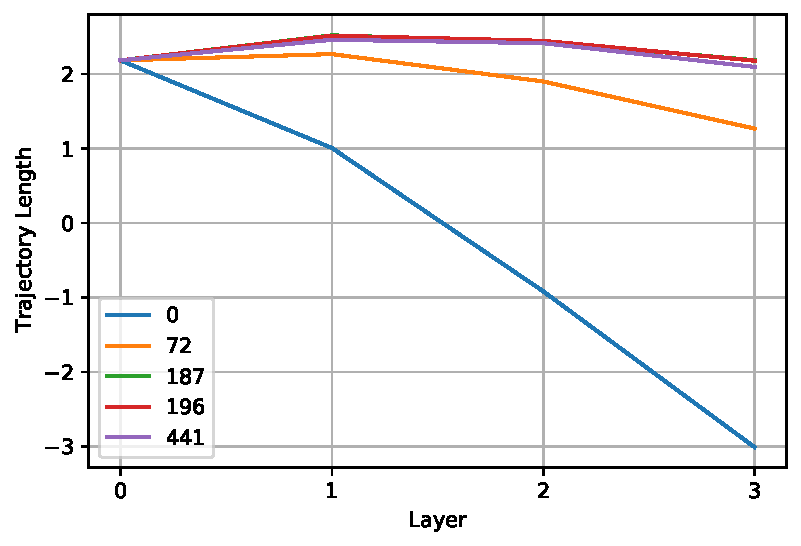
\includegraphics[height=1.9in]{latex/figures/TL_trained_DNN_nodes_9.pdf}
        \caption{Lorem ipsum}
    \end{subfigure}
    \caption{Caption place holder}
    \label{fig:TL_trained}
\end{figure}

From \autoref{fig:TL_trained}, we see that training the QCNs and DNNs progressively increases the trajectory length of the models. After only $10$ to $20$ epochs, the trajectory length of the 5 qubit QNC enters the exponential growth regime. This demonstrates that randomly initialized QCNs can be made to produce complex functions through training, even though outputs initially tended to concentrate around a mean, as shown in \autoref{fig:TL_untrained}. This shows that training updates the parameters in such a way that brings structure to each of the node QNNs, moving them away from being random circuits. This causes the outputs to no longer concentrate around the mean, which in turn lets the model compute more complex functions. As seen in (fig), 6-qubit is also eventually brought into the exponential growth regime(and strictly increasing with each layer) after between $50$ and $60$ epochs, which is significantly more than what was required for 5 qubits. As discussed in \autoref{sec:Vanishing Gradient Phenomenon}, increasing the number of qubits makes the magnitude of the gradient exponentially smaller. Thus, a larger number of epochs are required to significantly change the parameters such that the QNN nodes no longer resemble random circuits.

Moving over to the corresponding DNNs, we see that they fail to enter the same exponential growth regime as the QCNs, even when trained until they fit the data to the same degree. This indicates that QCNs, in this context, are more expressive than DNNs for the same number of parameters. Using the same argument as in \autoref{sec:Untrained Models}, the increased expressivity of QCNs relative to DNNs same number of parameters 

\begin{table}[H]
\centering
\begin{tabular}{|l|l|l|l|l|l|}
\hline
Model &Type & Qubits& Layers & Width &$n_{\theta}$ \\ \hline
A    & QCN & 5 &  3 & 5& 168   \\ \hline
B    & QCN & 6 &  3 & 6& 228 \\ \hline
C    & DNN & NA&  3 & 8& 177  \\ \hline
D    & DNN & NA&  3 & 9& 217  \\ \hline
\end{tabular}
\caption{Stuff.} 
\label{tab:TL models}
\end{table}



%================================================================
\section{Training Models on Gaussian Data}\label{sec:Training Models}
%================================================================
In this section, we will study various models in a more practical setting, fitting them to mixed Gaussian data in one, two and three dimensions. For more details on the data, see (see). We will train QNNs, QCN and DNNs with varying complexity and use MSE on the training data to evaluate how good the fit is. This will be done first in the ideal case, with exact calculation of outputs. Then, we will repeat the training for all models by simulating the noise model of the Santiago quantum computer(kilde). For a complete description of the models trained in this section, see \autoref{tab:training models}.

\begin{table}[H]
\centering
\begin{tabular}{|l|l|l|l|l|l|l|}
\hline
Model& Type& Data& Qubits& Layers & Width &$n_{\theta}$ \\ \Xhline{3\arrayrulewidth}
A    & QNN & 1D  & 4     & NA     & NA& 168   \\ \hline
B    & QCN & 1D  & 4     & 2      & 4& 228 \\ \hline
C    & QCN & 1D  & 4     & 2      & 4& 177  \\ \hline
D    & DNN & 1D  & NA    & 2      & 4& 217  \\ \Xhline{3\arrayrulewidth}
E    & QNN & 2D  & 4     & NA     & NA& 217  \\ \hline
F    & QCN & 2D  & 4     & 3      & 4& 217  \\ \hline
G    & QCN & 2D  & 4     & 3      & 4& 217  \\ \hline
H    & DNN & 2D  & NA    & 3      & 4& 217  \\ \Xhline{3\arrayrulewidth}
I    & QNN & 3D  & 5     & NA     & NA& 217  \\ \hline
J    & QCN & 3D  & 5     & 3      & 5& 217  \\ \hline
K    & QCN & 3D  & 5     & 3      & 5& 217  \\ \hline
K    & DNN & 3D  & NA    & 3      & 5& 217  \\ \hline
\end{tabular}
\caption{Stuff.} 
\label{tab:training models}
\end{table}


%================================================================
\subsection{Ideal Simulation}\label{sec:Ideal Simulation}
%================================================================
\autoref{fig:trained ideal} shows the MSE on the training data for the models defined in \autoref{tab:training models}, trained on the mixed Gaussian data. In order to produce a more significant result, each model is randomly initialized(see \autoref{sec:Initialization}) 10 times and trained separately. The resulting MSE for each model type is then averaged over the 10 runs and plotted with fill corresponding to one standard deviation. In this way, we get to see the average model behaviour during training  and how it varies between different runs.

\begin{figure}[H]
    \centering
    \begin{subfigure}[t]{0.5\textwidth}
        \centering
        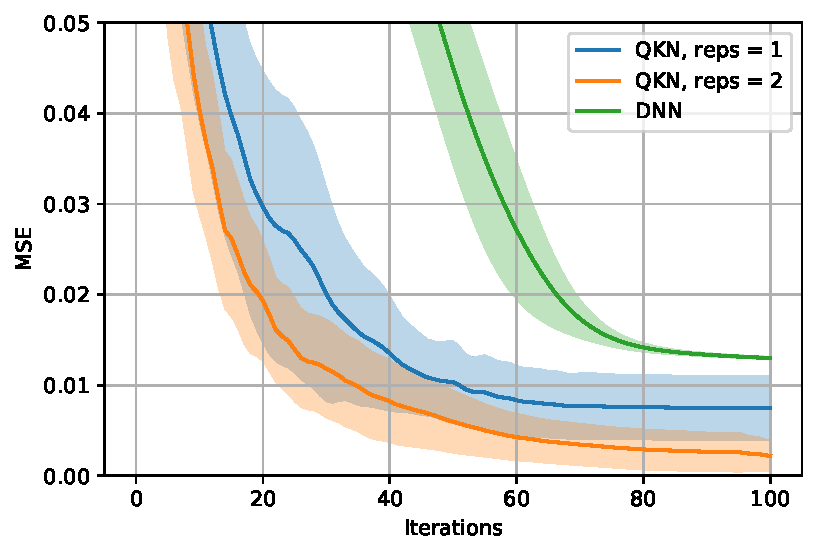
\includegraphics[height=1.9in]{latex/figures/1D_gaussian_data_fit.pdf}
        \caption{Lorem ipsum}
        
    \end{subfigure}%
    \hfill 
    \begin{subfigure}[t]{0.5\textwidth}
        \centering
        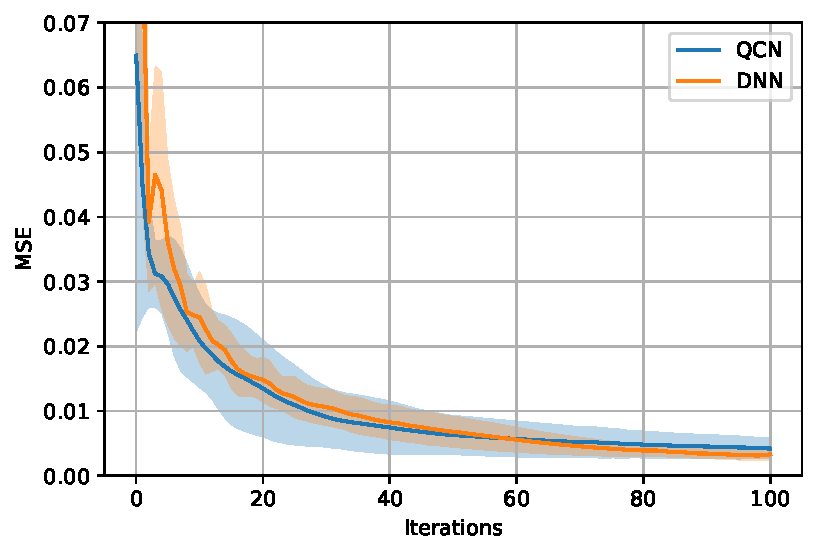
\includegraphics[height=1.9in]{latex/figures/2D_gaussian_data_fit.pdf}
        \caption{Lorem ipsum}
    \end{subfigure}
    \vskip\baselineskip
    \begin{subfigure}[t]{0.5\textwidth}
        \centering
        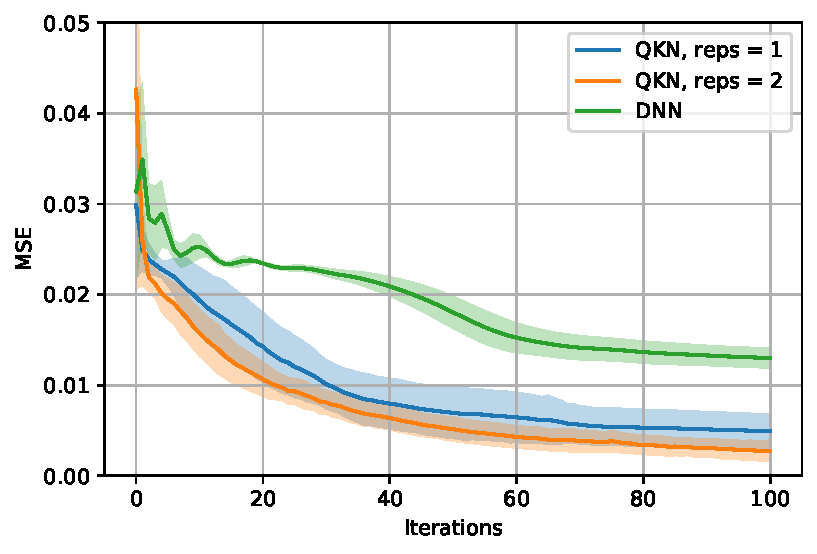
\includegraphics[height=1.9in]{latex/figures/3D_gaussian_data_fit.pdf}
        \caption{Lorem ipsum}
        
    \end{subfigure}%
    \caption{Caption place holder}
    \label{fig:trained ideal}
\end{figure}

From the above figure, we see that QCN models perform better than the other models on the Gaussian data. 
\begin{table}[H]
\centering
\begin{tabular}{|l|l|l|l|l|}
\hline
Model& Type& Data& MSE, $10^{2}$ Epochs& MSE, $10^{4}$ Epochs \\ \hline
A    & QNN & 1D  &    & NA   \\ \hline
B    & QCN & 1D  & $7.5\times 10^{-3}$  & NA \\ \hline
C    & QCN & 1D  & $2.2\times 10^{-3}$  & NA  \\ \hline
D    & DNN & 1D  & $1.3\times 10^{-2}$ & $5.1\times 10^{-5}$  \\ \Xhline{2\arrayrulewidth}
E    & QNN & 2D  &                    & NA  \\ \hline
F    & QCN & 2D  &                    & NA  \\ \hline
G    & QCN & 2D  &                    & NA  \\ \hline
H    & DNN & 2D  &                    &   \\ \Xhline{2\arrayrulewidth}
I    & QNN & 3D  &                    & NA  \\ \hline
J    & QCN & 3D  &                    & 5  \\ \hline
K    & QCN & 3D  &                    & 5  \\ \hline
K    & DNN & 3D  &                    & 5  \\ \hline
\end{tabular}
\caption{Stuff.} 
\label{tab:training models}
\end{table}

%================================================================
\subsection{Noisy Simulation}\label{sec:Noisy Simulation}
%================================================================

\begin{figure}[H]
    \centering
    \begin{subfigure}[t]{0.5\textwidth}
        \centering
        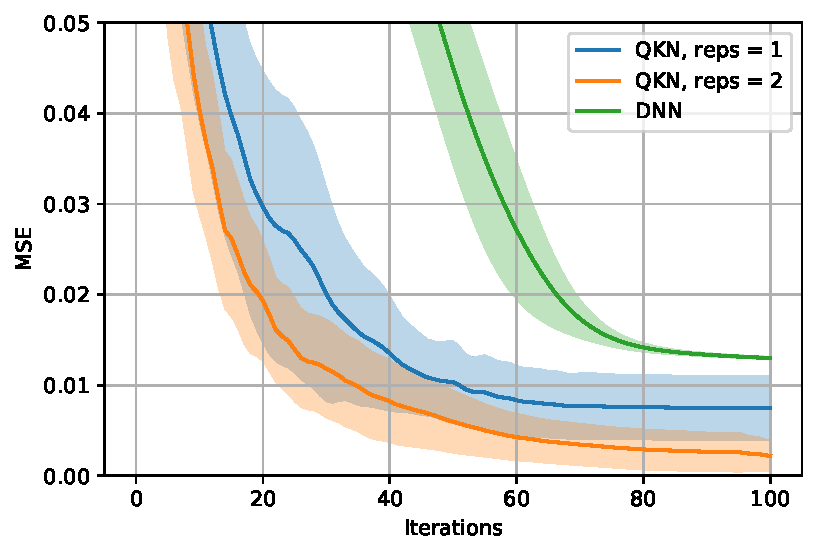
\includegraphics[height=1.9in]{latex/figures/1D_gaussian_data_fit.pdf}
        \caption{Lorem ipsum}
        
    \end{subfigure}%
    \hfill 
    \begin{subfigure}[t]{0.5\textwidth}
        \centering
        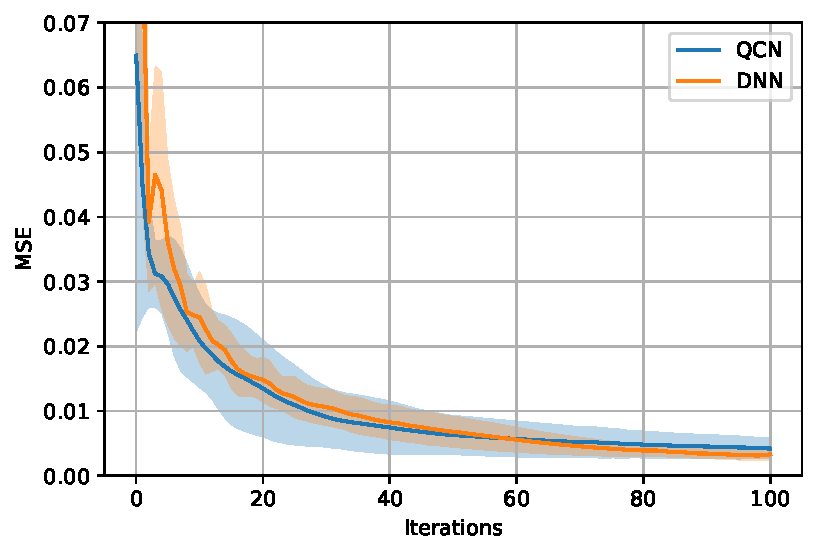
\includegraphics[height=1.9in]{latex/figures/2D_gaussian_data_fit.pdf}
        \caption{Lorem ipsum}
    \end{subfigure}
    \vskip\baselineskip
    \begin{subfigure}[t]{0.5\textwidth}
        \centering
        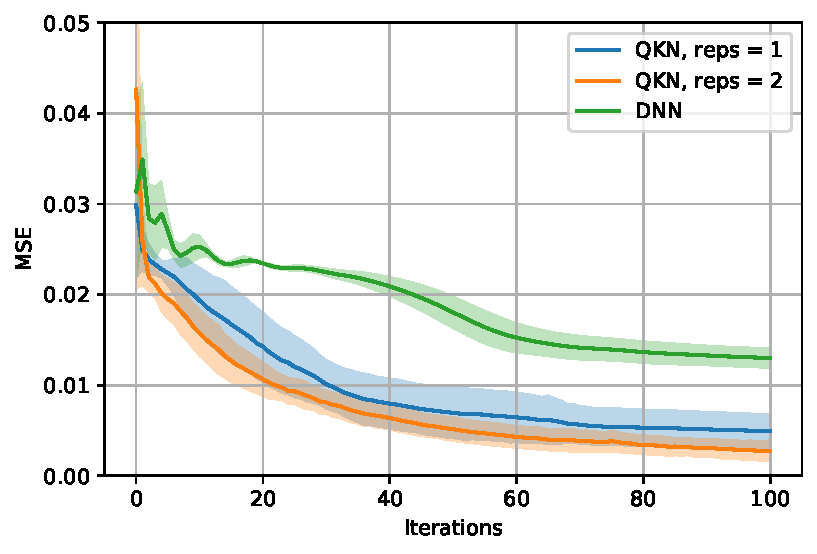
\includegraphics[height=1.9in]{latex/figures/3D_gaussian_data_fit.pdf}
        \caption{Lorem ipsum}
        
    \end{subfigure}%
    \caption{Caption place holder}
    \label{fig:trained ideal}
\end{figure}
